\begin{figure*}[t]
\centering
\begin{minipage}[t]{0.42\textwidth}
\centering
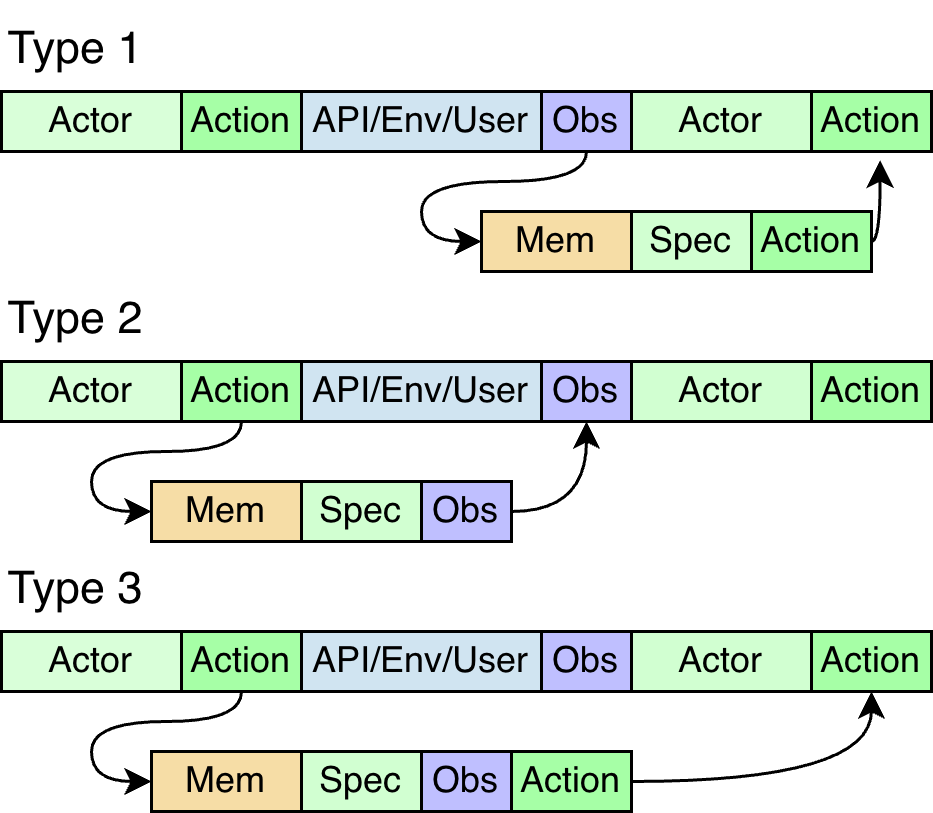
\includegraphics[width=\textwidth]{figures/method_left.png}
\end{minipage}%
\hfill
\begin{minipage}[t]{0.56\textwidth}
\centering
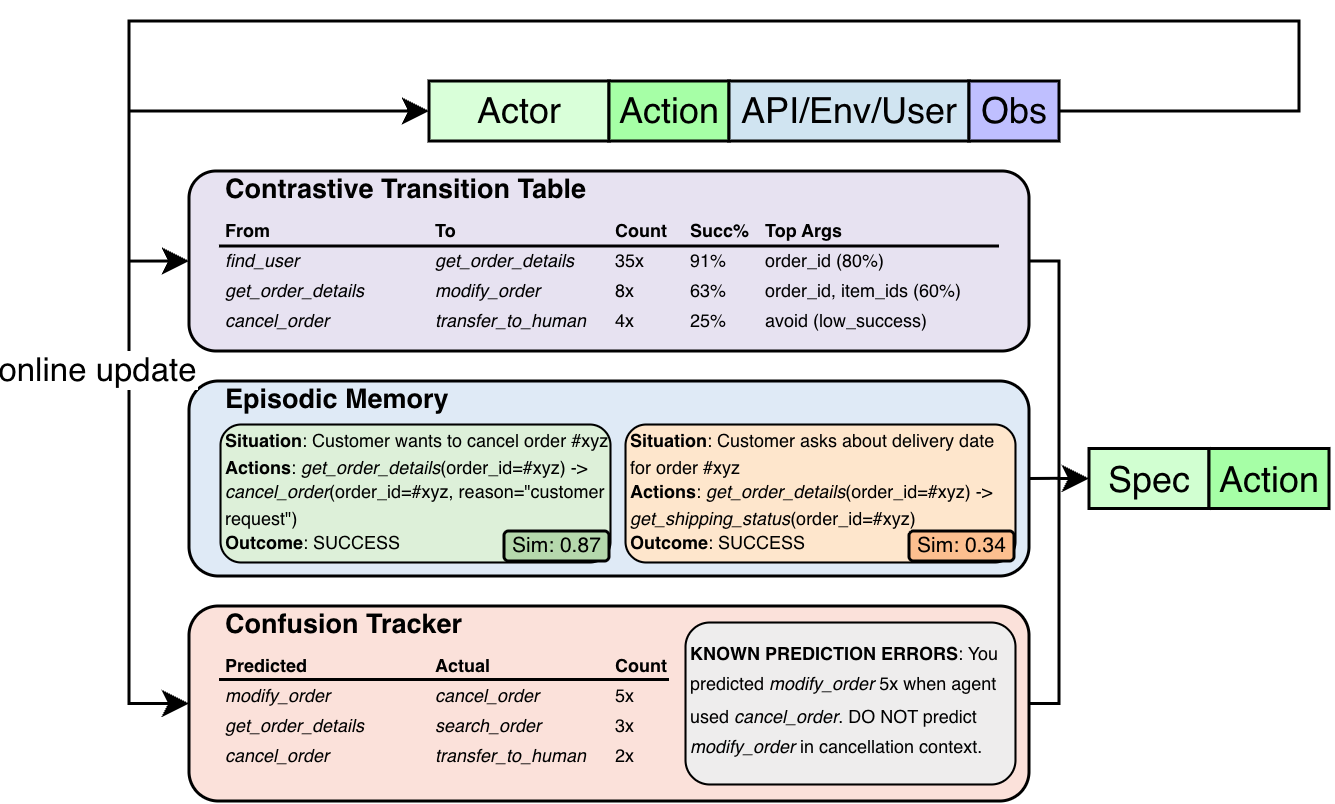
\includegraphics[width=\textwidth]{figures/method_right.png}
\end{minipage}
\caption{\textbf{Left:}~Timing of the three speculation types.  Each row
shows the agent-environment loop (top) and the speculator's parallel work
(bottom); shaded regions indicate saved latency on a hit.
\textbf{Right:}~Memory-augmented speculation architecture.  The agent loop
feeds online updates to three memory components (contrastive transition
table, episodic memory, and confusion tracker) that provide structured
context to the speculator.  Examples are from $\tau^{2}$-bench.}
\label{fig:method_overview}
\end{figure*}
